\documentclass[12pt,]{article}
\usepackage{lmodern}
\usepackage{setspace}
\setstretch{1.5}
\usepackage{amssymb,amsmath}
\usepackage{ifxetex,ifluatex}
\usepackage{fixltx2e} % provides \textsubscript
\ifnum 0\ifxetex 1\fi\ifluatex 1\fi=0 % if pdftex
  \usepackage[T1]{fontenc}
  \usepackage[utf8]{inputenc}
\else % if luatex or xelatex
  \ifxetex
    \usepackage{mathspec}
  \else
    \usepackage{fontspec}
  \fi
  \defaultfontfeatures{Ligatures=TeX,Scale=MatchLowercase}
\fi
% use upquote if available, for straight quotes in verbatim environments
\IfFileExists{upquote.sty}{\usepackage{upquote}}{}
% use microtype if available
\IfFileExists{microtype.sty}{%
\usepackage{microtype}
\UseMicrotypeSet[protrusion]{basicmath} % disable protrusion for tt fonts
}{}
\usepackage[margin = 1.18in]{geometry}
\usepackage{hyperref}
\PassOptionsToPackage{usenames,dvipsnames}{color} % color is loaded by hyperref
\hypersetup{unicode=true,
            pdftitle={Financial Fraud Detection Using Machine Learning Techniques},
            pdfauthor={Yordan Ivanov},
            colorlinks=true,
            linkcolor=black,
            citecolor=Blue,
            urlcolor=black,
            breaklinks=true}
\urlstyle{same}  % don't use monospace font for urls
\usepackage{longtable,booktabs}
\usepackage{graphicx,grffile}
\makeatletter
\def\maxwidth{\ifdim\Gin@nat@width>\linewidth\linewidth\else\Gin@nat@width\fi}
\def\maxheight{\ifdim\Gin@nat@height>\textheight\textheight\else\Gin@nat@height\fi}
\makeatother
% Scale images if necessary, so that they will not overflow the page
% margins by default, and it is still possible to overwrite the defaults
% using explicit options in \includegraphics[width, height, ...]{}
\setkeys{Gin}{width=\maxwidth,height=\maxheight,keepaspectratio}
\IfFileExists{parskip.sty}{%
\usepackage{parskip}
}{% else
\setlength{\parindent}{0pt}
\setlength{\parskip}{6pt plus 2pt minus 1pt}
}
\setlength{\emergencystretch}{3em}  % prevent overfull lines
\providecommand{\tightlist}{%
  \setlength{\itemsep}{0pt}\setlength{\parskip}{0pt}}
\setcounter{secnumdepth}{0}
% Redefines (sub)paragraphs to behave more like sections
\ifx\paragraph\undefined\else
\let\oldparagraph\paragraph
\renewcommand{\paragraph}[1]{\oldparagraph{#1}\mbox{}}
\fi
\ifx\subparagraph\undefined\else
\let\oldsubparagraph\subparagraph
\renewcommand{\subparagraph}[1]{\oldsubparagraph{#1}\mbox{}}
\fi

%%% Use protect on footnotes to avoid problems with footnotes in titles
\let\rmarkdownfootnote\footnote%
\def\footnote{\protect\rmarkdownfootnote}

%%% Change title format to be more compact
\usepackage{titling}

% Create subtitle command for use in maketitle
\newcommand{\subtitle}[1]{
  \posttitle{
    \begin{center}\large#1\end{center}
    }
}

\setlength{\droptitle}{-2em}
  \title{Financial Fraud Detection Using Machine Learning Techniques}
  \pretitle{\vspace{\droptitle}\centering\huge}
  \posttitle{\par}
  \author{Yordan Ivanov}
  \preauthor{\centering\large\emph}
  \postauthor{\par}
  \date{}
  \predate{}\postdate{}

\usepackage{booktabs}
\usepackage{longtable}

\begin{document}
\maketitle

\pagenumbering{roman}
\centering

\raggedright
\clearpage

\tableofcontents
\clearpage

\listoffigures
\clearpage

\listoftables
\clearpage

\hypertarget{variable-description}{%
\section{Variable Description}\label{variable-description}}

\(N\) - number of observations

\({\{(x_1,y_1),(x_2,y_2),...,(x_N,y_N)\}}\) - binary classification
dataset, N pairs of features and dependent variables

\(X\) - vector of features, with dimensions \(N\times p\)

\(y_i \in \{-1,1\}\) - scope of values which the dependent variable can
take

\(Y\) - vector of dependent variables (or classes), with dimensions
\(N\times1\)

\(\beta\) - coefficient produced by fitting logistic regression

\(w\) - weight vector normal to the hyperplane in SVM

\(\Phi\) - nonlinear mapping function

\(b\) - constant for the SVM algorithm

\(\xi\) - slack variable in SVM algorithm

\(C\) - misclassification cost in SVM algorithm

\(K(x_i,x_j)\) - kernel functions

\(\gamma\) - paramater in radial kernel function

\(B\) - number of bootstrapped datasets in Random Forest

\(Z^*\) - bootstrapped data sample

\(T_b\) - tree grown on bootstrapped data sample

\(s\) - randomly chosen subset of features

\(\Psi(y_i,\rho)\) - loss function

\(\rho\) - terminal nodes

\(\lambda\) - regularization parameter

\(F\) - number of nodes in neural network hidden layer

\clearpage

\pagenumbering{arabic}

\hypertarget{introduction}{%
\section{1.Introduction}\label{introduction}}

Financial fraud is an immense problem, resulting not only in billion
dollar losses each year, but also in long-term damage to corporate
reputation (Bhattacharyya et al. 2011; Fich and Shivdasani 2007). It is
undoubtedly among the biggest risks that business establishments face
today (Chaudhary and Mallick 2012). According to the 2014 ACFE report,
business organizations are suffering around 5\% revenue losses only due
to economic crime and fraud. Furthermore, financial fraud, and
especially credit card fraud, can be used to finance organized crime,
illegal drug trade groups or sometimes terrorist fractions (Everett
2003; McAlearney and Breach 2008). Thus, detecting financial fraud has
become more crucial than ever and the methods to do so need constant
innovation.

The remainder of the paper is organised as follows. In \emph{Section 2}
a background on financial fraud and e-commerce is provided. In the
subsequent section, a description of the six major machine learning that
are to be used is given. In \emph{Section 4}, the three datasets that
will be analyzed are presented and the problem of imbalanced classes is
reviewed. The next section is used to discuss the results obtained from
fitting the different machine learning techniques. \emph{Section 6}
briefly reviews what are the next steps for extending the scope of this
research. The final section includes an analysis of the findings that
this paper has produced.

\hypertarget{financial-fraud}{%
\section{2. Financial Fraud}\label{financial-fraud}}

\hypertarget{what-is-financial-fraud-and-e-commerce}{%
\subsection{2.1. What is Financial Fraud and
e-commerce?}\label{what-is-financial-fraud-and-e-commerce}}

The definition for fraud, as given by The Institute of Internal
Auditors' International Professional Practices Framework (IPPF), states:

``\ldots{} any illegal act characterized by deceit, concealment, or
violation of trust. These acts are not dependent upon the threat of
violence or physical force. Frauds are perpetrated by parties and
organizations to obtain money, property, or services; to avoid payment
or loss of services; or to secure personal or business advantage.''

Financial Fraud as a whole can be divided into two major categories -
Customer Fraud and Management Fraud (Bhardwaj and Gupta 2016). In this
paper, we will be focusing on Customer Fraud, or more precisely on
Credit Card and Transaction Fraud.

\begin{figure}
\centering
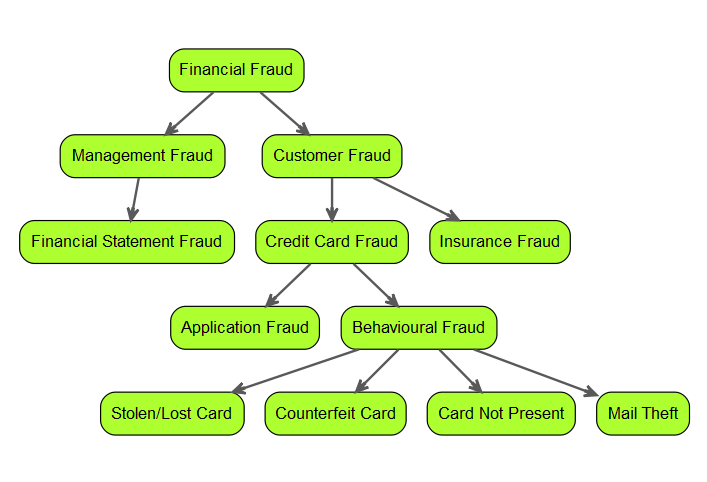
\includegraphics[width=0.7\textwidth,height=\textheight]{figures/fraud_hierarchy.png}
\caption{Financial Fraud Types}
\end{figure}

Credit Card can also be categorized in two groups - application and
behavioural fraud (Bolton and Hand 2001).The former category is
essentialy the acquisition of new cards from the issuing companies using
fraudulent or stolen information. The latter can be subcategorized into
stolen or lost card, counterfeit card, ``card not present'' fraud and
mail theft (See Figure 1). The stolen or lost card occurs when fraudster
manages to obtain physical posession of the card. The next two fraud
types, counterfeit and card not present, have been steadily rising in
numbers, thanks to the emergence of online transactions (Fletcher 2007).
Lastly, mail theft fraud occurs when the credit card is intercepted
before arriving by mail to the customer, or when fraudster steal
personal information from bank and credit card statements (One 2010).

Broadly speaking, e-commerce represents the business transactions that
are being made cyberspace, or ``Digitally enabled transactions'' (Laudon
and Traver 2013). There are five types of e-commerce -
business-to-commerce (B2C), business-to-business (B2B),
consumer-to-consumer (C2C), peer-to-peer (P2P) and mobile commerce
(m-commerce). The most vulnerable to fraud are B2C and C2C, as the main
reason is that in e-commerce the products and services can not be
inspected before the transaction is done (Grabosky, Smith, and Dempsey
2001). Hence, we have increased risks of fraud.

Thus, implementation of analytics that can scan through the transactions
being made is necessary for minimizing losses (Bănărescu 2015).

\hypertarget{costs-of-financial-fraud}{%
\subsection{2.2. Costs of Financial
Fraud}\label{costs-of-financial-fraud}}

Financial Fraud is currently one of the biggest threats to business
establishments, resulting in enormous finance losses each year. Only
throughout the year 2015, the losses from credit card fraud amounted to
\$21.84 Billion (Nilson 2016). Moreover, the losses occured by firms are
not only monetary - damage on reputation and customer ties could prove
to be devastating (ACL 2014). Thus, the overall losses from financial
fraud are simply incalculable (Ngai et al. 2011).

\hypertarget{combating-financial-fraud-and-related-work}{%
\subsection{2.3. Combating Financial Fraud and Related
Work}\label{combating-financial-fraud-and-related-work}}

As a result from the increase in the amount of data globally, there has
also been a rise in the use of predictive analytics (Bănărescu 2015).
When talking about financial fraud, the forensic data analytics (FDA)
are being used, but the percentage of sophisticated methods and software
applied is not very high (See Table 1). A big percentage of the industry
uses spreadsheet tools or database tools, which in their nature are
primitive in terms of data analysis.

\begin{table}

\caption{\label{tab:table analytics}Forensic Data Analysis Tools in use}
\centering
\fontsize{8}{10}\selectfont
\begin{tabular}[t]{ll}
\toprule
Forensic.Data & Percent\\
\midrule
Spreadsheet tools such as MS Excel & 65\%\\
Database tools such as MS Access or MS SQL Server & 43\%\\
Continious monitoring tools  (SAP, Oracle, SAI Global) & 29\%\\
Text analytics tools or keyword searching & 26\%\\
Forensic analytics software (ACL, iDEA) & 26\%\\
\addlinespace
Social media/web monitoring tools & 21\%\\
Visualization and reporting tools (Tableau, Spotfire,                                                     QlikView) & 12\%\\
Statistical analysis and data-mining packages (R,                                                        SAS, Stata, SPSS) & 11\%\\
Big data technologies (Hadoop, Map Reduce) & 2\%\\
Voice searching and analysis (Nexidia, NICE) & 2\%\\
\bottomrule
\multicolumn{2}{l}{\textsuperscript{a} Source [@analytics\_tools\_table]}\\
\end{tabular}
\end{table}

In the report by EY (2014), the respondents state that by using more
complicated and proactive methods, they have faced a 59,7\% reduction in
median loss, in comparison to the respondents that did not.

Among the more complex and successful methods for fraud reduction are
machine learning (ML) techniques (Chaudhary and Mallick 2012). The ML
models used for FFD, and especially credit card fraud, can be broadly
categorized into two major groups - supervised and unsupervised learning
methods. The unsupervised techniques depend only on the characteristics
of each transaction, grouping them into clusters with homogenous
attributes. Whenever an observation is not assigned to an already
existing cluster of legal transactions, it signals that there is a
probability that the transaction is fraudulent (Bolton and Hand 2001).
However, most studies in the field have focused on the use of supervised
learning methods for FFD (Ngai et al. 2011). In this framework, the
model is trained on already labeled datasets, recognizing the patterns
associated with fraudulent transactions. Among the techniques most used
for credit card are logistic regression, support vector machines (SVM),
artificial neural networks (ANN), bayesian networks, and different tree
models (Ngai et al. 2011; Bhattacharyya et al. 2011; Chaudhary and
Mallick 2012).

The focus on this paper will be on supervised learning methods. In the
literature, a greater focus has been put on supervised methods (Ngai et
al. 2011), but the overall are of fraud detection has not been
thoroughly explored, due to the sensitivity and public unavailaibility
of datasets (Dal Pozzolo and Bontempi 2015). In the studies that have
been done, the overall focus has been on ANNs. Among the first to adopt
an ANN approach to the problem of FFD are Ghosh and Reilly (1994),
through the use of a P-RCE ANN - a three layer and feed-forward network.
The method employed had relative success, identifying correctly on
average 40\% of the fraud. The ANN is since then among the most used
methods for FFD. Brause, Langsdorf, and Hepp (1999) and Dorronsoro et
al. (1997) have achieved better results with an ensemble method
including ANNs. However, ANNs have been, and still are, considered as
black-box models and are hard to interpret. Thus, other methods, such as
random forest, have risen in popularity and have also shown impressive
performance in the field of FFD (Bhattacharyya et al. 2011; Dal Pozzolo
et al. 2014). Logistic Regression is also quite popular, especially due
to its strong interpretability, but can sometimes lack the prediction
power of other, more complex ML algorithms (Bhattacharyya et al. 2011).
The SVM has also been employed, due to its advantages in terms of solid
theoretical foundations. However, the results produced by the methods
have been mixed, mainly because the FFD problem poses an imbalanced
class challenge (Chaudhary and Mallick 2012; Bhattacharyya et al. 2011).
Nonetheless, it has been shown that through changes in the foundations
of the SVM method, in order to transform to model into a cost-sensitive
one, better performance can be achieved on problems with imbalanced data
(He and Garcia 2009).

Slightly surprising is that almost no research about the performance of
boosting methods has been made in the field of FFD, especially credit
card fraud, given the capabilities of ML models such as stochastic
gradient boosting machines and eXtreme gradient boosting (Nielsen 2016;
Chen and Guestrin 2016). We will deploy both methods in order to compare
their performances against the other, more established, frameworks.

\hypertarget{methodology}{%
\section{3. Methodology}\label{methodology}}

Classification is one of the most widely used model framework used for
the application of machine learning techniques in terms of FFD (Ngai et
al. 2011). Some of the most common classification techniques include
logistic regression, neural networks, support vector machine and
decision trees and their variations.

\hypertarget{preliminaries}{%
\subsection{3.1. Preliminaries}\label{preliminaries}}

In the current section, we will give a description of the machine
learning techniques that we apply to predict fraudulent transactions.

Let us define our binary classification dataset as
\({\{(x_1,y_1),(x_2,y_2),...,(x_N,y_N)\}}\), where
\(x_i\in \mathbb{R}^n\) represents an n-dimensional data point and
\(y_i \in \{-1,1\}\) represents the label of the class of that data
point, \(i = 1,...,p\). Let \(X\) represent the vector of features and
\(Y\) the vector of dependent variables.

\hypertarget{machine-learning-algorithms}{%
\subsection{3.2. Machine Learning
Algorithms}\label{machine-learning-algorithms}}

\hypertarget{logistic-regression}{%
\subsubsection{3.2.1. Logistic Regression}\label{logistic-regression}}

The logistic regression framework falls under the category of
generalized linear models and allows the prediction of discrete
outcomes. Then, by defining the probability of a transaction being
fraudulent by \(p(X) = Pr(Y=1|X)\), we can portray the relationship
between the dependent and independent variables as follows:

\[p(X) = \frac{e^{\beta_0 + \beta_1X_1 + ... + \beta_pX_p}}{1 + e^{\beta_0 + \beta_1X_1 + ... + \beta_pX_p}}\;\;\;\;(1)\]

The number of independent variables is indexed by \emph{p}. After
manipulating (1), we can also see that
\[log(\frac{p(X)}{1-p(X)})=\beta_0+ \beta_1X_1 + ... + \beta_pX_p\;\;\;\;(2)\]
with the LHS being called the logit. Using equation (2), we will predict
the probabilities of a transaction being fraudulent i.e. \(p(Y = 1)\).
The fitting of a logistic regression is done by the method of maximum
likelihood. The logistic regression has been among the most widely used
framework in fraud detection (Ngai et al. 2011) due to simplicity of
ease of implementation, but it does have its shortcomings - it tends to
underperform when there are multiple or non-linear decision boundaries.

\hypertarget{neural-networks}{%
\subsubsection{3.2.2. Neural Networks}\label{neural-networks}}

Neural Networks is a term that currently describes a wide array of
different algorithms. However, we will be using the ``vanilla'' version,
which contains only a single hidden layer, but this can be extended to
include more {[}friedman2001elements{]}. However, that is beyond the
scope of this paper.

A feed-forward neural network with one hidden layer can be seen in
Figure 1. It has \(g\) outputs nodes, which in our case would be
\(g=2\), as we are dealing with two-class classification problem. Each
output node would give us the probability of an observation belonging to
a specific class.

\begin{figure}
\centering
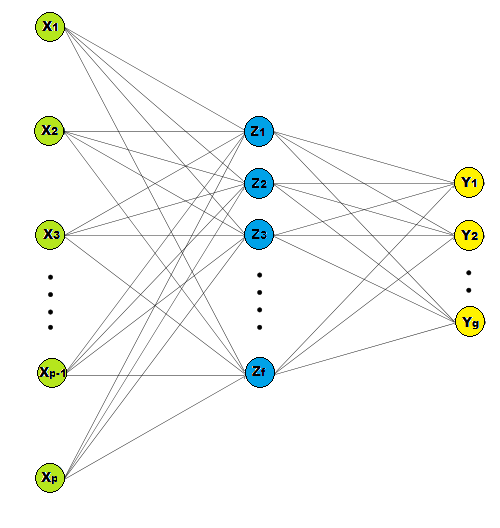
\includegraphics[width=0.6\textwidth,height=\textheight]{figures/nnet.png}
\caption{Neural Network with 1 hidden layer}
\end{figure}

The features \(Z_f\) are being derived through linear combinations of
the inputs, while the \(Y_g\) outputs are then modeled as a function of
linear combinations of the \(Z_m\), or mathematically formulated as
follows:

\[Z_f=\sigma(\alpha_{0f}+\alpha_{m}^{T}X),\;f=1,...,F\]
\[T_g=\beta_{0g}+\beta_{k}^{T}Z,\;g=1,2\] \[f_{g}(X)=g_g(T),\;g=1,2\]

where \(T=(T_1,T_2)\), \(Z=(Z_1,Z_2,...,Z_F)\) and
\(g_g(T)=\frac{e^{T_g}}{\sum_{f=1}^{F}e^{T_f}}\) represents the softmax
function. We use the sigmoid activation function
\(\sigma(v)=\frac{1}{1+e^{-v}}\). In order to fit the neural network and
estimate the set of weights \(\{\alpha_{0f},\alpha_{f};f=1,2,3...,F\}\)
and \(\{\beta_{0g},\beta_{g},g=1,2\}\), we use the backpropagation
equations in order to minimize the error term.

\hypertarget{support-vector-machines}{%
\subsubsection{3.2.3. Support Vector
Machines}\label{support-vector-machines}}

Support Vector Machines, developed by Vapnik et. al. (Cortes and Vapnik
1995), have become a popular machine learning method that has seen its
implementation rise in various domains that require the use of
classification models (Batuwita and Palade 2013). Among the factors for
its success is the fact that the SVMs are linear classifiers, which work
in a high-dimensional feature that represents a non-linear mapping of
the input space of the problem being dealt with (Bhattacharyya et al.
2011). Working in a high-dimensional feature space has its benefits -
often, the problem of non-linear classification in the original input
space is transformed to a linear classification task in the
high-dimensional feature space.

The goal of the SVM classifier consists of finding the optimal
separating hyperplane, which manages to effectively separate the
observations from the data into two classes. As mentioned above, the
observations are initially transformed by a nonlinear mapping function
\(\Phi\). Thus, we can write a possible separating hyperplane that
resides in the transformed higher dimensional feature space by:

\[w\cdot\Phi(x)+b=0\;\;\;\;(3)\] with \(w\) the weight vector normal to
the hyperplane.

We will further use two variations of the SVM soft margin optimization
problem - one that assigns the same cost for missclassification of the
different classes and one that penalizes more the missclassification of
the minority class.

\hypertarget{non-cost-sensitive-learning}{%
\paragraph{Non-cost sensitive
learning}\label{non-cost-sensitive-learning}}

For the same missclassification cost case, we can write the soft
optimization problem as follows:
\[\min(\frac{1}{2}w \cdot w + C\sum_{i=1}^{p} \xi_i) \]
\[s.t. \;\; y_i(w \cdot \Phi(x_i) + b) \geq 1 - \xi_i\;\;\;\;(4) \]
\[\xi_i \geq 0, i = 1,...,p\] The slack variables \(\xi_i > 0\) hold for
missclassified examples. Thus, the penalty term \(\sum_{i=1}^{p}\) can
be perceived as the total number of missclassified observations of the
model. Thus from (4), we can see that there are two goals - maximizing
the margin the minimizing the number of missclassifications. The cost
parameter C controls the trade-off between them, i.e.~assigned
misclassification cost. The quadratic optimization problem in (4) can be
represented by a dual Lagrange problem and then solved:
\[\max_{\alpha_i} \{ \sum_{i=1}^{p}{\alpha_i} - \frac{1}{2} \sum_{i=1}^{p}\sum_{j=1}^{p}{\alpha_i\alpha_j\Phi(x_i)\cdot\Phi(x_j)} \} \;\; s.t. \;\; \sum_{i=1}^{p}{y_i\alpha_i}=0, \;\; 0 \leq\alpha_i\leq C, \;\; i=1,...,p\;\;\;\;(5) \]

\(\alpha_i\) are the Lagrange multipliers also satisfying the
Karush-Kuhn-Tucker (KKT) conditions (see Appendix). Thanks to another
one of the strenghts of SVM - kernel representation - we don't need to
explicitly know the mapping function \(\Phi(x)\), but by applying a
kernel function (i.e. \(K(x_i,x_j) = \Phi(x_i)\cdot \Phi(x_j)\)), we can
rewrite (5) as:
\[\max_{\alpha_i} \{ \sum_{i=1}^{p}{\alpha_i} - \frac{1}{2} \sum_{i=1}^{p}\sum_{j=1}^{p}{\alpha_i\alpha_jK(x_i,x_j)} \} \;\; s.t. \;\; \sum_{i=1}^{p}{y_i\alpha_i}=0, \;\; 0 \leq\alpha_i\leq C, \;\; i=1,...,p\;\;\;\;(6)\]
The solution then gives us \(w = \sum_{i=1}^{p}{\alpha_iy_i}\phi(x_i)\)
for the optimal values of \(\alpha_i\) and \(w\), while \(b\) is
determined from KKT. The data points that have \(\alpha_i\) different
than zero are called the support vectors. Thus, the decision function
can be written was:
\[f(x) = sign(w \cdot \Phi(x) + b) = sign(\sum_{i=1}^{p}{\alpha_iy_i}K(x_i,x_j) + b)\;\;\;\;(7) \]

\hypertarget{cost-sensitive-learning}{%
\paragraph{Cost Sensitive learning}\label{cost-sensitive-learning}}

The regular SVM model has been effectively implemented when the dataset
used has balanced classes, however it fails to produce good results when
applied on imbalanced data (Batuwita and Palade 2013). When trained on a
dataset with extremely imbalanced classes, the SVM framework could
produce so skewed hyperplances that all observations are recognized as
the majority class (Akbani, Kwek, and Japkowicz 2004,
@veropoulos1999controlling). This is due to the fact that when we take
the soft margin optimization problem, we try to maximize the margin and
minimize the penalty for the misclassifications. As we consider a
constant C for all training examples, the minimization of the penalty is
achieved through the minimization of all misclassifications. However,
when the used dataset suffers from imbalanced classes, the majority
class density would be higher than the minority class density, even when
considering the class boundary region (through which the ideal
hyperplane would pass).

Thus, we consider here the application of the Different Error Costs
(DEC) variation of the SVM algorithm proposed by Veropoulos et al.
(1999). The DEC method introduces different misclassification costs -
\(C^+\) for the minority and \(C^-\) for the majority class. With the
inclusion of the higher misclassification cost for the minority class
observations, the imbalanced class effect could be brought down. The
soft margin optimization problem then has the following form:
\[\min{(\frac{1}{2}w \cdot w + C^+\sum_{i|y_i=+1}^{p}\xi_i + C^-\sum_{i|y_i=-1}^{p}\xi_i)}\]
\[s.t. \;\; y_i(w \cdot \Phi(x_i) + b) \geq 1 - \xi_i\;\;\;\;(8)\]
\[\xi_i \geq 0, i = 1,...,p\] The Dual Lagrange optimization form is the
same as before, with the exception of replacing \(0 \leq\alpha_i\leq C\)
with \(0 \leq\alpha_i^+\leq C^+, \; 0 \leq\alpha_i^-\leq C^-\) for
\(i=1,...,p\). The \(\alpha_i^+\) and \(\alpha_i^-\) are the Lagrange
multipliers. The solution of the DEC dual Lagrangian problem follows the
same outline as in the normal form.

\hypertarget{kernels}{%
\paragraph{Kernels}\label{kernels}}

As mentioned before, we used a kernel function
(\(K(x_i,x_j) = \Phi(x_i)\cdot \Phi(x_j)\)) in order to transform the
dual Lagrange problem. The advantages of using kernel functions are
computational or in some cases it allows for computations that otherwise
would be impossible (James et al. (2013)). For the purpose of this
study, we are using the linear and radial kernels. The radial kernel
shows good performance on non-linear class separation. They have the
following representations:
\[Linear: \;\;\; K(x_i,x_j) = \sum_{k=1}^{l}x_{ik}x_{jk}\;\;\;\;(9)\]
\[Radial: \;\;\; K(x_i,x_j) = exp(-\gamma\sum_{k=1}^{l}(x_{ik}-x_{jk})^2), \;\; \gamma=\frac{1}{2\sigma^2}\;\;\;\;(10)\]

\hypertarget{tree-based-methods}{%
\subsubsection{3.2.4. Tree-Based Methods}\label{tree-based-methods}}

Tree-based methods involve segmentation of the feature space into a set
of regions and then fitting a simple model to each one. Even though are
not too complex conceptually, they are still a very powerful method (J.
Friedman, Hastie, and Tibshirani 2001). Firstly, we will give a short
overview of a standard classification decision tree (DT) before moving
on the methods used in this study.

Let us call the set of non-overlapping regions \(R_1,R_2,...,R_M\) that
are used to divide the feature space. The forms of those regions are
high-dimensional rectangles - for simplicity and interpretability. The
aim for DT would be to find the boxes that minimize the error term,
which in the case of classification can be represented in several ways -
misclassification error, Gini index or cross-entropy. However, it is
very computationally taxing to consider every feasible partition of the
feature space into \(M\) boxes. Thus, the recursive binary splitting
method is used, which is a top-down, greedy approach - it starts at the
top of the tree and then it splits the feature space, making the best
split possible, without looking forward. The algorithm is further
described in the Appendix.

However, the beforementioned algorithm can sometimes lead to
over-fitting and producing very ineffecient prediction results. Thus,
the tree pruning technique is applied - first a large tree is grown,
then it is ``pruned'' and a smaller version is obtain. The procedure
leads to reduction in variance at the cost of some bias. Usually the
cost complexity pruning algorithm is used in practice - a more thorough
description is included in the Appendix.

The regular classification DT has high interpretability, but it
sometimes lacks sufficient prediction power - they are often unstable
and can be too sensitive to training data (Bhattacharyya et al. 2011).
This leads us to variations of the classic classification DT.

\hypertarget{random-forests}{%
\paragraph{Random Forests}\label{random-forests}}

A random forest algorithm is an ensemble of classification trees
(Breiman 2001). The model starts with growing each tree on separate
bootstrapped dataset. Moreover, only a randomly selected feature subset,
typically \(s \simeq \sqrt{p}\) (Khoshgoftaar, Golawala, and Van Hulse
2007), is used at each individual node. As a result, the entire
algorithm is based on two basic, yet powerful, concepts - bagging and
random subspace method. To better illustrate the random forest method,
the pseudo-algorithm is given below:

\emph{Algorithm Random Forest}

\begin{enumerate}
\def\labelenumi{\arabic{enumi}.}
\tightlist
\item
  For \(b\) = 1 to \(B\) (\(B\) is representing the number of
  bootstrapped datasets):

  \begin{itemize}
  \tightlist
  \item
    Draw bootstrapped sample \(Z^*\) of size \(N\) from the dataset used
    for training
  \item
    Grow a RF tree \(T_b\) on the previously bootstrapped dataset by
    recursively looping the below given steps for each tree terminal
    node, up until the \(n_{min}\) node (minimum size node) is reached:

    \begin{itemize}
    \tightlist
    \item
      Select \(s\) features randomly from the entire feature subset,
      \(p\).
    \item
      Choose the best available variable/split-point among the \(s\).
    \item
      Split node into two children nodes.
    \end{itemize}
  \end{itemize}
\item
  Output the tree ensemble \(\{T_b\}^{B}_{1}\).
\item
  Making the prediction for a new point \(x\): If \(\widehat{C}_b(x)\)
  is the prediction of the class for the \(b\)th RF tree, then
  \(\widehat{C}_{rf}^{B}(x)=majority\;vote\{\widehat{C}_b(x)\}_{1}^{B}\).
\end{enumerate}

The Random Forest algorith has been quite popular lately, due to its
simplicity and performance. It has only two parameters that can be
changed - the number of trees grown and the size of the feature subset
used (Breiman 2001). Furthermore, it has often shown superior
performance to one if its rival statistic learning method - the SVM
(Meyer, Leisch, and Hornik 2003). In the area of financial fraud
detection, RF has also shown to be a promising framework (Whitrow et al.
2009, @ngai2011application).

\hypertarget{stochastic-gradient-boosting-machines-and-extreme-gradient-boosting-machines}{%
\paragraph{Stochastic Gradient Boosting Machines and eXtreme Gradient
Boosting
Machines}\label{stochastic-gradient-boosting-machines-and-extreme-gradient-boosting-machines}}

The ideas introduced by the boosting methodology have been among the
most influential in the last twenty years (J. Friedman, Hastie, and
Tibshirani 2001). Among the most used and influential boosting
algorithms is ``AdaBoost.M1'' (Freund and Schapire 1997). It was the
first developed ``adaptive'' boosting algorithm, due to its incorporated
function to directly adjust its parameters to the used training dataset.
This is due to the fact, that the performance of the model was
re-evaluated at each iteration - the parameters weights and the final
aggregated weights, were re-calculated and improved at each iteration,
thus leading to an overall better performance. Moreover, it was found
that not only AdaBoost, but boosting algorithms in general, managed to
not only reduce variance, but also bias - an improvement over bagging,
where only the variance could be decreased.

The followwing success led to the formulation and development of the
gradient-descent based methods, which received the name gradient
boosting machines or simply GBM (Freund and Schapire 1997; Friedman et
al. 2000; J. H. Friedman 2001). The general idea of GBMs is to fit new
models iteratively, constructing the base-learners to be maximally
correlated with the loss function's negative gradient, in order to get a
better estimate of the response variable (Natekin and Knoll 2013).
Moreover, the algorithm offers flexibility in terms of choosing the form
of the loss function. In this study, we use the Bernoulli distribution,
as we are dealing with a two-class classification problem.

Due to its flexibility and ease of implementation, the GBM algorithm has
proven to be a successful model, that offers high predictive power when
dealing with machine learning problems (Whiting et al. 2012,
@johnson2014learning). Furthermore, when including a random element in
the algorithm, as in the Stochastic GBM (SGBM), results tend to improve
(Friedman 2002). We describe the pseudo-code of the SGBM for a two-class
problem below.

\emph{Stochastic Gradient Tree Boosting Machines (Stochastic GBM)}

Two-Class Classification as in the \textbf{gbm} R package.

\begin{enumerate}
\def\labelenumi{\arabic{enumi}.}
\item
  Initialize \(f_{0}(x) = \arg\min_{\rho}\sum_{i=1}^{N}\Psi(y_i,\rho)\).
\item
  For \(m=1\) to \(M\) do:

  \begin{itemize}
  \tightlist
  \item
    Compute negative gradient:
    \[z_{im}=-\frac{\partial{\Psi(y_{i},f(\mathbf{x}_i))}}{\partial{f(\mathbf{x}_i)}}\rvert_{f(\mathbf{x}_i)=\widehat{f}(\mathbf{x}_i)},\; i=1,...,N\]
  \item
    Randomly select \(s \times N\) subset.
  \item
    Fit regression tree with K number of terminal nodes on the
    previously selected subset, \(g(\mathbf{x})=E(z|\mathbf{x})\).
  \item
    Compute the optimal terminal node predictions,
    \(\rho_{1m},...,\rho_{Km}\), as:
    \[\rho_{km}=\arg\min_{\rho}\sum_{\mathbf{x}_i \in S_k} \Psi(y_i,\widehat{f}(\mathbf{x}_{i})+\rho_k)\],
    where \(S_k\) is the set of \(\mathbf{x}\)'s that define terminal
    node \(k\).
  \item
    Compute
    \(\widehat{f}_{m}(x)=\sum_{k=1}^{K}\rho_{km}I(x_i\in\widehat{R}_{km})\),
    as \(\{\widehat{R}_{km}\}_{k=1}^{K}\) represents the tree structure.
  \item
    Update \(\widehat{f}^{m}(\mathbf{x})\) as
    \(\widehat{f}^{m}(\mathbf{x}) \leftarrow \widehat{f}_{m-1}(\mathbf{x}) + \lambda\widehat{f}_{m}(x)\).
  \end{itemize}
\item
  Output \(\widehat{f}(x) = f_{M}(x)\)
\end{enumerate}

The eXtreme Gradient Boosting algorithm, or shortly XGBoost, was
developed as an attempt to improve on the performance of GBM, both in
terms of speed and prediction power (Chen and Guestrin 2016). It has has
not only succeeded in doing so, but it has also become one of the most
used models (Nielsen 2016). Among the differences that XGBoost
introduces in comparison to the GBM model is that the former uses clever
penalization of the individual trees - the leaf weights are not all
decreased at the same rate, instead the weights which are estimated
without much evidence from the training set will be shrunk more heavily
relative to others. Furthermore, the XGBoost employs another type of
boosting structure when compared to GBM - Newton boosting. Due to this,
the algorithm manages to better learn tree structures, leading to
learning better neighbourhoods. XGBoost also incorporates a
randomization paramater, which contributes to the individual tree
decorellation and reducing variance. Some technical detail references
regarding the differences between XGBoost and GBM are included in
Appendix 9.1 - such as the gradient and Newton boosting and leaf weight
learning. The general pseudo-codes are similar.

\hypertarget{cross-validation}{%
\subsection{3.3. Cross-Validation}\label{cross-validation}}

The framework for model training that we use in this study is a
\(k\)-fold Cross-Validation (CV) with \(k=10\) (James et al. 2013). The
method incorporates a random division of the training set into \(k\)
folds with approximately similar size. The initial fold is used a
validation set and the chosen statistical learning model is fit on the
remaining \(k-1\) folds. The error is then calculated on the
observations in the held-out fold. The entire process is then repeated
\(k\) times, with a different validation set at each iteration, thus
computing \(k\) estimates of the test error. The \(k\)-fold CV estimate
can then be shown as: \[CV_{(k)}=\frac{1}{k}\sum_{i=1}^{k}Err_i\] where
\(Err_i = I(y_i\neq \widehat{y}_i)\).

There are other approaches to CV, such as the Leave-One-Out CV (LOOCV),
but the \(k\)-fold CV has shown to be superior in both computational
time and estimate accuracy (J. Friedman, Hastie, and Tibshirani 2001).
The latter is connected to the bias-variance trade-off problem, but a
discussion is out of the scope of this paper. A graphical representation
can be seen in Figure 1 in Appendix Section 9.4.

\hypertarget{data}{%
\section{4. Data}\label{data}}

\hypertarget{datasets}{%
\subsection{4.1. Datasets}\label{datasets}}

The number of datasets that we will be using in this study is three -
two real-world and one simulated. Each dataset has been randomly
splitted to two - a train and a test subset. The train consists of 60\%
of the original dataset, while the test the remaining 40\%.

\hypertarget{real-world-datasets}{%
\subsubsection{4.1.1. Real-World Datasets}\label{real-world-datasets}}

\hypertarget{ucsd-fico-data-mining-contest-2009}{%
\paragraph{UCSD-FICO Data Mining Contest
2009}\label{ucsd-fico-data-mining-contest-2009}}

The dataset was released by FICO, one of the leading analytics
providers, and the University of California, San Diego (UCSD). It
consists of real-world e-commerce transactions and it was released in
two versions - an ``easy'' and a ``hard'' one. We will be using the
``hard'' version for the assessments of the models used. Due to the
fact, that is a real-world data set, anonymiziation is introduced, which
means that methods depending on feature aggregation or feature
engineering will not lead to improvement in efficiency (Seeja and
Zareapoor 2014). Nonetheless, some data preprocessing is done.

The dataset consists of 100 000 transactions made by 73 729 different
customers throughout 98 days. Each transaction is characterized by 20
features - amount, hour1, state1, zip1, custAttr1, field1, custAttr2,
field2, hour2, flag1, total, field3, field4, indicator1, indicator2,
flag2, flag3, flag4, flag5. It can be observed that custAttr1 is the
customer card number, while the custAttr2 is the e-mail address. As both
fields are unique, we discard custAttr2. The other unique feature pairs
per customer are the amount/total, hour1/hour2 and state1/zip1, thus
discarding total, hour2 and state1 leaves us with 16 fields.

Furthermore, customers with just one transaction have been removed,
leaving us with 40 918 transactions. Only 2.922\% of the transactions
are fraudulent, which indicates severe imbalacedness.

\hypertarget{universite-libre-de-bruxelles-ulb-machine-learning-group}{%
\paragraph{Université Libre de Bruxelles (ULB) Machine Learning
Group}\label{universite-libre-de-bruxelles-ulb-machine-learning-group}}

The dataset was released by the Université Libre de Bruxelles (ULB)
Machine Learning Group and it consists of real-world credit card
transactions made throughout two days from the year 2013 (Dal Pozzolo et
al. 2015). Strong anonymization is introduced, as the entire dataset has
gone through a Principal Component Analysis (PCA) transformation.

The number of transactions included are 284 807 with 30 features
characterizing each one. The only two labeled features are Time and
Amount, while all 28 others are numericals resulting from the PCA. We do
not do any feature engineering, as there is no information on what each
column represents.

The number of frauds is just 492, which means only 0.172\% of all
transactions are positively labeled, indicatin very severe class
imbalance. However, we will work with 100 000 randomly selected
observations, as to decrease the computation time. The fraudulent
observation still represent only 0.187\% of all transactions.

\hypertarget{simulated-datasets}{%
\subsubsection{4.1.2. Simulated Datasets}\label{simulated-datasets}}

Due to lack of publicly available datasets on real-world fraud, the
simulation of such has become important (Lopez-Rojas and Axelsson 2014).
Thus, we will use two generated sets in order to evaluate the chosen
statistical learning methods and gather more data on their performance
in the area.

\hypertarget{paysim}{%
\paragraph{PaySim}\label{paysim}}

The first synthetic dataset that we will use originates from a simulator
called PaySim, which was developed by Lopez-Rojas and Axelsson (2014).
It represents a simulation based on an e-commerce payment platform for
making payments through a mobile device.

The generated dataset is constructed thanks to an agent-based-simulation
application, which uses real-world information. It consists of nine
features - step, type, amount, nameOrig, oldbalanceOrg, newbalanceOrig,
nameDest, oldbalanceDest and newbalanceDest. The step represents a
time-stamp, the type shows what kind of transaction occurs, nameOrig and
nameDest give us unique ID's of the sender and receiver of the
transaction, while the rest oldbalanceOrg, newbalanceOrig,
oldbalanceDest and newbalanceDest represent the amount present in the
accounts of the sender and receiver before and after the financial
transaction has been made. Furthermore, we introduce some feature
engineering by creating two more variables - errorBalanceOrig and
errorBalanceDest. The errorBalanceOrig is generated by summing up
newbalanceOrig and amount and then subtracting oldbalanceOrg. The
motivation behind this is that a positive errorBalanceOrig could be a
fraud pattern, due to an amount of being lost along the line of the
transaction. Analogcally, the errorBalanceDest has the some concept
behind it, but for the destination account.

Overall, the dataset consists of 6 362 620 observations, but only
0.129\% of them are fraudulent, indicating very severe classimbalance.
Due to the large size of the dataset and the computationally-demanding
methodology that we are using, only a 100 000 observation subset will be
used.

\hypertarget{problems-of-imbalanced-data-and-data-sampling-techniques}{%
\subsection{4.2. Problems of Imbalanced Data and Data Sampling
Techniques}\label{problems-of-imbalanced-data-and-data-sampling-techniques}}

\hypertarget{problem-of-imbalanced-data}{%
\subsubsection{4.2.1. Problem of Imbalanced
Data}\label{problem-of-imbalanced-data}}

One of the biggest challenges faced in detecting fraudulent transactions
is the one of unbalanced class sizes, with legitimate class outnumbering
vastly the fraudulent one (Bhattacharyya et al. 2011). The application
of data-sampling techniques has been widely used in the literature with
various results when combined with different algorithms, as when such a
problem occurs, it could hinder the model performances (Van Hulse,
Khoshgoftaar, and Napolitano 2007). Moreover, in our particular case,
the cost of missclassifying the minority class could prove to be a lot
more costly than predicting wrongly the majority one.

\hypertarget{data-sampling-techniques}{%
\subsubsection{4.2.2. Data Sampling
Techniques}\label{data-sampling-techniques}}

\hypertarget{random-oversampling-rosand-random-undersampling-rus}{%
\paragraph{Random Oversampling (ROS)and Random UnderSampling
(RUS)}\label{random-oversampling-rosand-random-undersampling-rus}}

The two techniques are the simplest and most common (Van Hulse,
Khoshgoftaar, and Napolitano 2007). In minority oversampling (ROS), the
observations from the minority group are randomly duplicated in order to
balance the dataset. In majority undersampling (RUS), the aim is the
same, but it is achieved by randomly removing observations of the
majority class.

\hypertarget{weighted-dataset}{%
\paragraph{Weighted Dataset}\label{weighted-dataset}}

The technique for weighting your dataset is to closes thing to achieving
a cost-sensitive learning model through manipulating the raw dataset.
Class weights are chosen between the model is fit on the data and
usually the minority class is given greater importance than the majority
one, thus pays more ``attention'' when learning. \emph{FIND SOURCES FOR
THIS}

\hypertarget{smote}{%
\paragraph{SMOTE}\label{smote}}

The Synthetic Minority Oversampling Technique (SMOTE), proposed by
Chawla et al. (Chawla et al. 2002), artificial minority instances are
created not simply through duplication, but rather with the
extrapolation between preexisting observations. The technique starts by
taking into account the k nearest neighbourhoods to a minority
observation for every instance from that class. Then, the artificial
observation are created, taking into account just a part of the nearest
neighbours or all of them (with respect to the desired oversampling
specification).

\hypertarget{results}{%
\section{5. Results}\label{results}}

\hypertarget{performance-measures}{%
\subsection{5.1. Performance Measures}\label{performance-measures}}

As the problem that we deal with in this paper is a classification one,
the performance measures used to evaluate how successful a model will be
related to the main building block of binary classification - the
confusion matrix.

\begin{longtable}[]{@{}lll@{}}
\toprule
. & Actual.Positive & Actual.Negative\tabularnewline
\midrule
\endhead
Predicted Positive & True Positive (TP) & False Positive
(FP)\tabularnewline
Predicted Negative & False Negative (FN) & True Negative
(TN)\tabularnewline
\bottomrule
\end{longtable}

\hypertarget{threshold-metrics}{%
\subsubsection{5.1.1. Threshold Metrics}\label{threshold-metrics}}

\[Sensitivity = \frac{TP}{TP + FN}\;\;\;\;\;\;Specificity =\frac{TN}{FP+TN} \]
The sensitivity of a given classifier indicates what percent of the
positive class has been actually predicted as positive. Analogically,
specifity gives the percent of the negative class which has been
assigned as negative by the model. Overall, the measures give us a
picture of the proportions that have been correctly predicted.

\[Precision = \frac{TP}{TP+FP}\;\;\;\;\;\;Recall=\frac{TP}{TP+FN}\] The
precision measure indicates how well the used classifier identifies a
given class' observation, i.e.~checks the percent of the observations
assigned a positive class that are truly positive. The recall
formulation is same as the sensitivity one. Both measures are typically
used together in order to get more information about the positive class.

\[F_\alpha=\frac{(1+\alpha)[precision \times recall]}{[\alpha\times precision] + recall}\]
The F-measure falls to the category of combination metrics and its
purpose is to combine the precision and recall in a single scalar. One
of its advantages is that allows us to weight the two components as
desired through the \(\alpha\) component. Usual values of \(\alpha\) are
\(0.5, 1\) or \(2\) - with \(1\) we specify that precision and recall
are equal in weights, \(2\) indicates precision is twice as important as
recall and \(0.5\) gives two times more weight to recall. When dealing
with class imbalanace, the F-measure can give more in-depth insight
(Japkowicz 2013).

\hypertarget{ranking-methods-and-metrics}{%
\subsubsection{5.1.2. Ranking Methods and
Metrics}\label{ranking-methods-and-metrics}}

\hypertarget{roc-curve-analysis}{%
\paragraph{ROC Curve Analysis}\label{roc-curve-analysis}}

The Receiver-Operating-Characteristic, or simply ROC, is a simple, yet
very powerful tool. The ROC curve is created by using the False
Posititve Rate (FPR) and Sensitivity (or True Positive Rate (TPR)) and
plotting them against each at different threshold settings. The FPR is
defined as \(FPR=\frac{FP}{FP+TN}\). An example ROC curve can be seen in
Figure 3. The better the line ``hugs'' the upper left corner of the ROC
space, the better the trained classifier is. A model that produces a
line that is close to the 45-degree separator means that it does not
perfor better than random guessing.

\begin{figure}
\centering
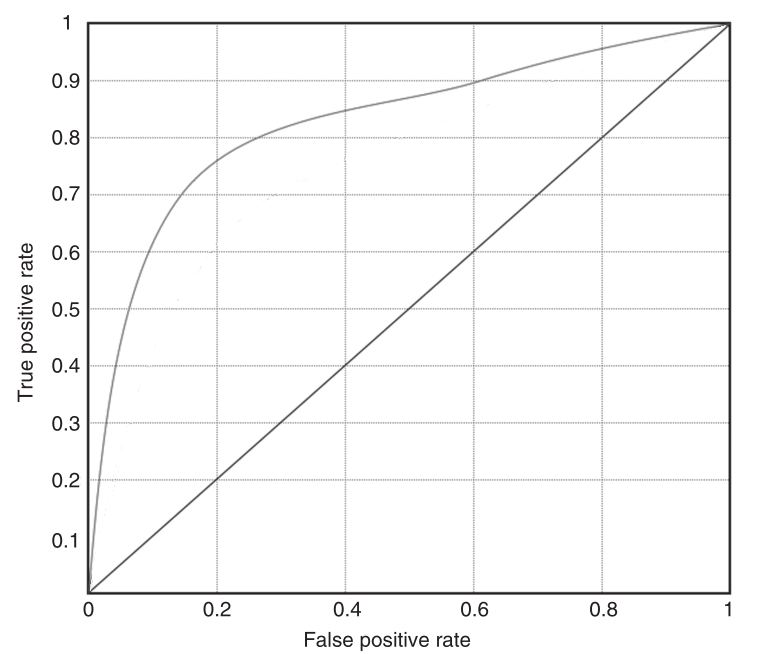
\includegraphics[width=0.6\textwidth,height=\textheight]{figures/roc_curve_example.png}
\caption{Well performing ROC curve example}
\end{figure}

Moreover, when dealing with imbalanced classes, the ROC metric is a very
suitable indicator of whether a model is a good fit. The first reason is
that we have the performance of each class shown separately (through the
two axes) and the second one is that it gives a good overview what can
happen in different situations (Japkowicz 2013).

\hypertarget{precision-and-recall-curve-analysis}{%
\paragraph{Precision and Recall Curve
Analysis}\label{precision-and-recall-curve-analysis}}

The Precision and Recall (PR) Curve Analysis is very similar to ROC
Curve Analysis, as it once again gives an overview of the
correctly-classified positive class and and the number of
incorrectly-classified negative observations. However, the PR curve
plots, as expected, the precision and recall on the two axes, showing
the various states the precision metric can take given different levels
of recall. Unlike the ROC curve, the PR one has a negative slope, due to
the fact precision decreases with the increase of recall. There have
been suggestions that PR curves can be more informative than ROC curves
when working with imbalanced classes (Davis and Goadrich 2006).

\hypertarget{area-under-curve-auc}{%
\paragraph{Area-Under-Curve (AUC)}\label{area-under-curve-auc}}

The AUC metric illustrates the performance of a classification model
averaged over all of the feasible cost ratios. Given that the ROC curve
operates in a unit square, it can be seen that the AUC in this case
could take values only between 0 and 1, i.e. \(AUC \in [0,1]\), with
\(AUC=1\) representig the perfect classifier and \(AUC=0.5\) the random
one. It can be argued that the AUC is a good summary metric that can
assess the performance of a classifier and be used for comparisons, but
it too loses significant information over the entire operating range
(for instance trade-off behaviour between TP and FP performances).

\hypertarget{experimental-results}{%
\subsection{5.2. Experimental Results}\label{experimental-results}}

We have conducted all experiments on a machine running 4GB RAM, Intel(R)
Core(TM) i3-2330M CPU @ 2.20GHz or on the Kaggle Cloud Computing
Service, where depending on the statistical model that was geing
calculated, up to 32 cores and 17 GB RAM were utilized. The programming
software that we used was R - R Studio on the local machine and R
scripts on the cloud.

We will use 10-fold Cross-Validation in order to tune the model
parameters and will use the ROC as an optimization criterion, as it is
argued that it is a good indicator when dealing with imbalanced classes
(He and Garcia 2009). The Accuracy metric will be used as little as
possible to determine a classifier performance, as even if a model fails
to classify a single observation from the minority class, the accuraccy
will still be high (and close to 100\% in some cases, due to sever class
imbalance). Thus the ROC and AUC metrics will be utilized in order to
gauge the performances and choose the optimal machine learning
technique.

As we apply six different machine learning techniques to each dataset
and we have at least five variations of each technique, we will present
in detail only the comparison between different models and not between
each model variation. The model variation included in the final
comparison will be the one that has exhibited the best performance. For
details on model tuning and variable importance, see Appendix.

The different variations executed involve fitting the model with
different data-sampling techniques , i.e.~each model is fitted using the
original dataset, RUS set, ROS set, SMOTE set and a weighted dataset.

\hypertarget{ucsd}{%
\subsubsection{5.2.1. UCSD}\label{ucsd}}

As mentioned in \emph{Section 4.1.1.}, we wil work with 40 918
observations. As this is a real dataset and its features are mostly
masked, this means that there is no real feature engineering that we can
perform before applying any machine learning techniques.

From the 40 918 observations, only 1 196 are fraudulent. Hence, there is
not much that we derive from our raw data and that can be observed from
the graphics created to illustrate the distribution of the different
features (See Appendix). The only interesting note that can be taken is
that it seems the fraudulent class is usually associated with a
transaction that has a lower amount. This can be seen in Figure 4.

\begin{figure}
\centering
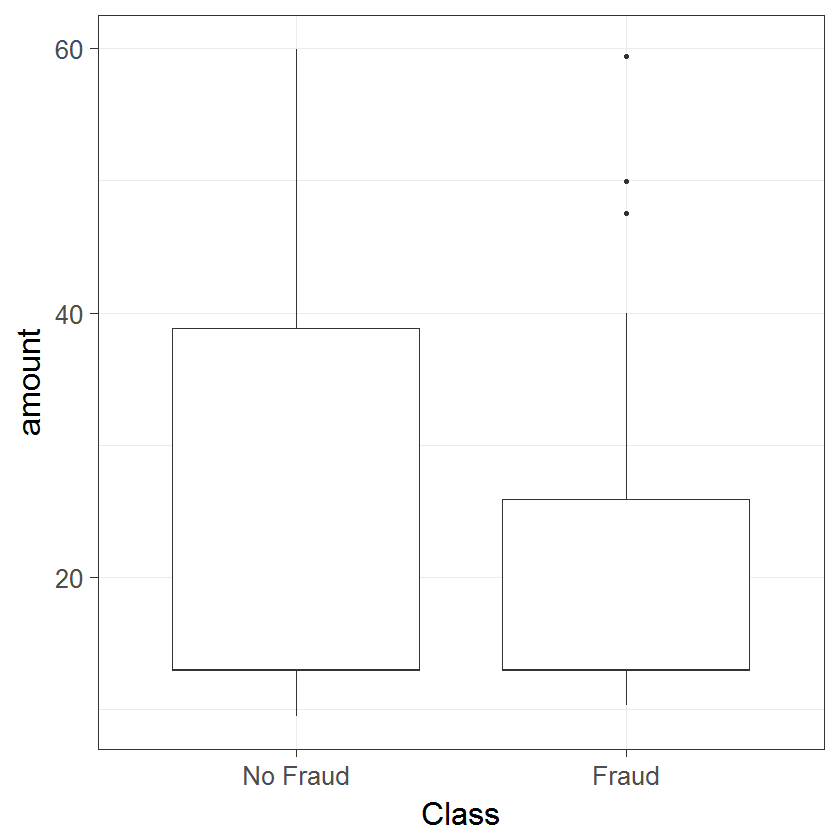
\includegraphics[width=0.6\textwidth,height=\textheight]{figures/ucsd/descriptive/boxplot_amount.png}
\caption{Boxplot of amount by class}
\end{figure}

However, when we turn to the ML Techniques, patterns seem to arise and
better predictions can be made. We first shortly present the 10-fold
Cross-Validation results that were obtained from fitting the models on
the dataset variations. In Tables 3 and 4, we can observe ROC AUC and
Precision-Recall AUC of the models that were used in this study.

\begin{table}

\caption{\label{tab:ucsd_models_AUC}UCSD: AUC Metric Model Variations}
\centering
\resizebox{\textwidth}{!}{\begin{tabular}[t]{lrrrrrrr}
\toprule
type & original & original\_radial & weighted & weighted\_radial & down & up & SMOTE\\
\midrule
Random Forest & 0.8548012 & NA & 0.8548012 & NA & 0.8168893 & 0.8651387 & 0.8356639\\
xGBoost & 0.8218285 & NA & 0.8227247 & NA & 0.8055749 & 0.8249255 & 0.8031042\\
GBM & 0.7765399 & NA & 0.7739591 & NA & 0.7542527 & 0.7754709 & 0.7446644\\
ANN & 0.7188902 & NA & 0.7133446 & NA & 0.6970364 & 0.7083888 & 0.7015769\\
Log. Regression & 0.6902922 & NA & NA & NA & 0.6862027 & 0.6892931 & 0.6896683\\
SVM & 0.6324302 & 0.730891 & 0.6416904 & 0.7320982 & 0.6985871 & 0.6898714 & 0.7131695\\
\bottomrule
\end{tabular}}
\end{table}

\begin{table}

\caption{\label{tab:ucsd_model_PR}UCSD: PR Metric Model Variations}
\centering
\resizebox{\textwidth}{!}{\begin{tabular}[t]{lrrrrrrr}
\toprule
type & original & original\_radial & weighted & weighted\_radial & down & up & SMOTE\\
\midrule
Random Forest & 0.5151509 & NA & 0.5151509 & NA & 0.3515450 & 0.4591128 & 0.4062699\\
xGBoost & 0.4242364 & NA & 0.4247124 & NA & 0.2055611 & 0.3885884 & 0.2906456\\
GBM & 0.2831942 & NA & 0.1773567 & NA & 0.1419057 & 0.1937535 & 0.1461725\\
ANN & 0.0985339 & NA & 0.0860225 & NA & 0.0691229 & 0.0960196 & 0.0749699\\
Log. Regression & 0.0780961 & NA & NA & NA & 0.0783426 & 0.0735142 & 0.0681947\\
SVM & 0.0574525 & 0.164502 & 0.0597058 & 0.164611 & 0.0712216 & 0.0667245 & 0.0783384\\
\bottomrule
\end{tabular}}
\end{table}

It is quite evident from these two tables that the best performing model
throughout each setting is Random Forests. Unsurprisingly, it is
followed by the eXtreme Gradient Boosting, which also produces really
good results. The SVM is also expectedly suffering, due to the severe
class imbalance, which as mentioned in Section 3, leads to the support
vector being pushed close to the majority class, thus ignoring the
minority. The Logistic Regression performs relatively competitive and
having a huge computational speed advantage means it is in no way
irrelevant.

In Figure 5 we also visually show the differences between the different
Machine Learning Techniques. Here it is also quite evident that the
Random Forest method shows superiority. Its ROC curve is higher than all
the other at every point, while the Precision Recall curve is lower than
the weighted xGBoost only in a very limited range.

\begin{figure}
\centering
\includegraphics[width=1\textwidth,height=\textheight]{figures/ucsd/ucsd_pr_roc.png}
\caption{UCSD: ROC and PR Curves}
\end{figure}

\hypertarget{credit-card}{%
\subsubsection{5.2.2. Credit Card}\label{credit-card}}

As discussed in \emph{Section 4.1.1.}, we wil work with a subset of 100
000 bservations. Due to the fact that this a real-world dataset and has
PCA performed on it in order to hide any private information, we can not
perform any feature engineering or informative descriptive data
analysis.

One of the few things that we can observe by exploring our data is that
the fraud class has fewer observation that are associated with very
large amounts. That can be seen in Figure 6, where we show a boxplot of
all transaction with amount less than 2000 in order to better illustrate
the beforementioned statement.

\begin{figure}
\centering
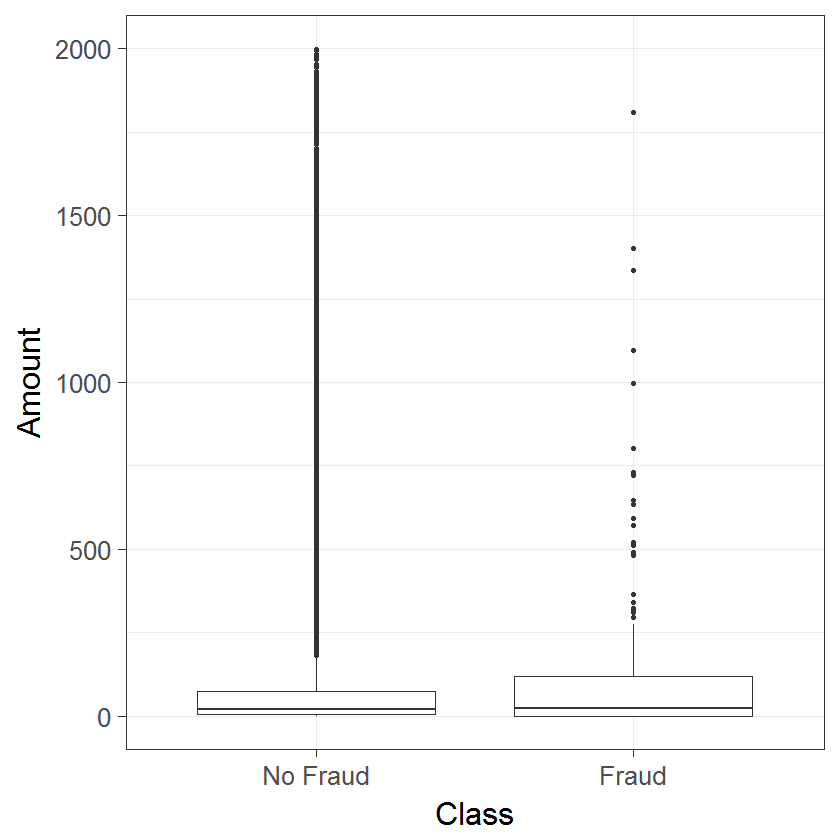
\includegraphics[width=0.6\textwidth,height=\textheight]{figures/credit/descriptive/cr_card_fraud_amount_boxplot.png}
\caption{Boxplot of amount by class in Credit Card Dataset}
\end{figure}

However, when applying the ML Techniques discussed in \emph{Section 3},
we are better able to use our data for analysing and prediction. In
Tables 5 and 6, we can see the ROC AUC and Precision-Recall AUC of the
different models and the different data-sampling techniques. The fitting
framework is once again 10-fold Cross-Validation.

\begin{table}

\caption{\label{tab:cr_card_models_AUC}Credit Card: AUC Metric Model Variations}
\centering
\resizebox{\textwidth}{!}{\begin{tabular}[t]{lrrrrrrr}
\toprule
type & original & original\_radial & weighted & weighted\_radial & down & up & SMOTE\\
\midrule
Random Forest & 0.9543801 & NA & 0.9543801 & NA & 0.9682755 & 0.9542050 & 0.9638472\\
xGBoost & 0.9692195 & NA & 0.9668218 & NA & 0.9456119 & 0.9771028 & 0.9673158\\
GBM & 0.5805464 & NA & 0.9744766 & NA & 0.9703028 & 0.9690840 & 0.9659266\\
ANN & 0.9639963 & NA & 0.9737695 & NA & 0.9708280 & 0.9554879 & 0.9567426\\
Log. Regression & 0.9443036 & NA & NA & NA & 0.8141654 & 0.8967922 & 0.9088207\\
SVM & 0.9181649 & 0.9592933 & 0.9247987 & 0.9627719 & 0.9181649 & 0.9181649 & 0.9181649\\
\bottomrule
\end{tabular}}
\end{table}

\begin{table}

\caption{\label{tab:cr_card_model_PR}Credit Card: PR Metric Model Variations}
\centering
\resizebox{\textwidth}{!}{\begin{tabular}[t]{lrrrrrrr}
\toprule
type & original & original\_radial & weighted & weighted\_radial & down & up & SMOTE\\
\midrule
Random Forest & 0.8330339 & NA & 0.8330339 & NA & 0.7927356 & 0.8527693 & 0.8110314\\
xGBoost & 0.8336317 & NA & 0.8068010 & NA & 0.5619452 & 0.7535501 & 0.7895484\\
GBM & 0.4362846 & NA & 0.8202291 & NA & 0.4189344 & 0.8358836 & 0.5228063\\
ANN & 0.7773746 & NA & 0.7618862 & NA & 0.3955604 & 0.5590176 & 0.6677604\\
Log. Regression & 0.7584590 & NA & NA & NA & 0.0089959 & 0.7249762 & 0.0375165\\
SVM & 0.7810338 & 0.7322844 & 0.7719868 & 0.7437641 & 0.7810338 & 0.7810338 & 0.7810338\\
\bottomrule
\end{tabular}}
\end{table}

From the two tables, 5 and 6, we can observe that all models perform
relatively similar. However, Random Forest and xGBoost are one step
above the rest, in both the ROC AUC and Precision-Recall AUC metrics.
The SVM also manages to predict better than expected, despite dealing
with sever class imbalance. Nonetheless, it's Non Cost-Sensitive variant
is still the worst performing model. On this dataset we can see how the
inclusion of different costs in the SVM algorithm for the different
class classification manages to improve performance. Both cost-sensitive
variants, using linear or radial kernel, outperform the ``vanilla'' SVM.

In Figure 7, both left and right, we can see the red, green and
sometimes pink line, representing RF, xGBoost and GBM respectively, are
slightly above all others. One all these three models have in common, is
that they are based on the principle of decision trees. They do employ
different fitting algorithm, bagging and boosting, but still perform on
a similar high level.

\begin{figure}
\centering
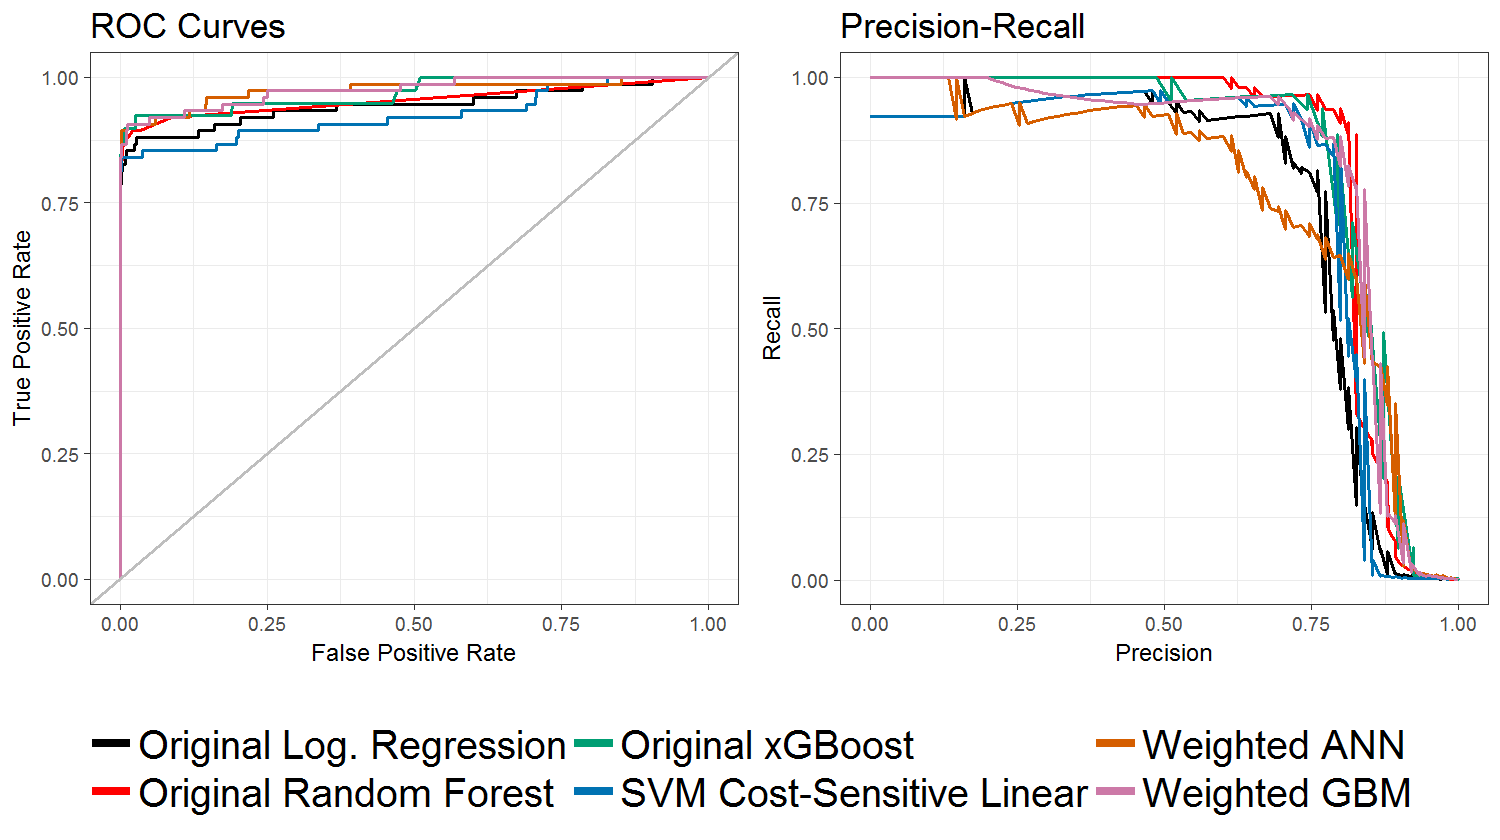
\includegraphics[width=1\textwidth,height=\textheight]{figures/credit/cr_card_roc_pr.png}
\caption{Credit Card: ROC and PR Curves}
\end{figure}

\hypertarget{paysim-1}{%
\subsubsection{5.2.3. PaySim}\label{paysim-1}}

As we have examined in \emph{Section 4.1.2.}, the features contained in
the PaySim are not masked and thus some descriptive data analysis can be
made. Moreover, as mentioned, we have created two more features, which
are based on the ones already existing in the PaySim file -
errorBalanceOrig and errorBalanceDest. The errorBalanceOrig was created
by summing up newbalanceOrig and amount and then subtracting
oldbalanceOrg. Analogically, errorBalanceOrig is the summation of
newbalanceDest and amount, then subtracting oldbalanceDest.

\begin{table}

\caption{\label{tab:paySim_fraud_types}PaySim: AUC Metric Model Variations}
\centering
\fontsize{8}{10}\selectfont
\begin{tabular}[t]{lrr}
\toprule
type & isFraud & freq\\
\midrule
CASH\_IN & 0 & 21979\\
CASH\_OUT & 0 & 34914\\
CASH\_OUT & 1 & 64\\
DEBIT & 0 & 698\\
PAYMENT & 0 & 33968\\
\addlinespace
TRANSFER & 0 & 8316\\
TRANSFER & 1 & 61\\
\bottomrule
\end{tabular}
\end{table}

\begin{figure}
\centering
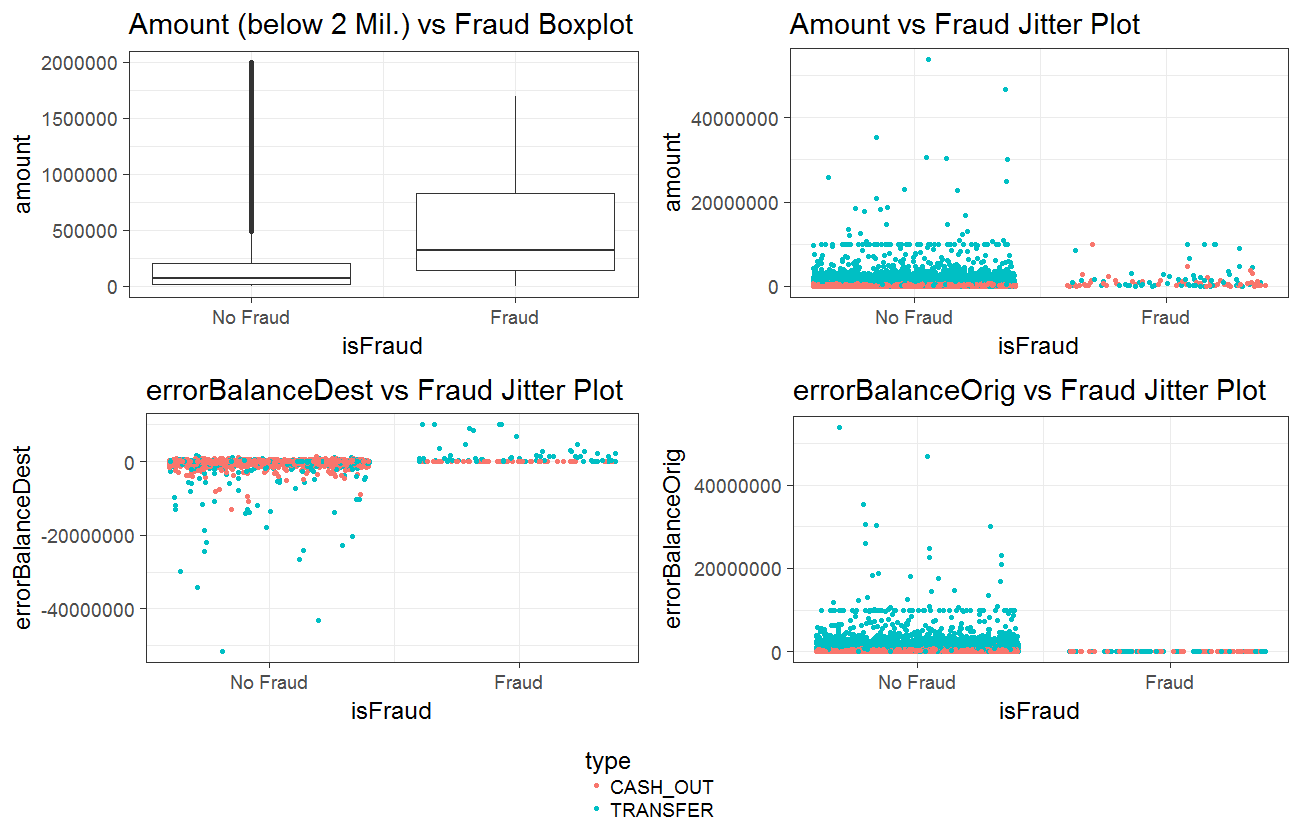
\includegraphics[width=0.9\textwidth,height=\textheight]{figures/paySim/descriptive/four_plots.png}
\caption{PaySim: Exploratory Data Analysis Plots}
\end{figure}

On Table 7, it can be clearly seen that fraud occurs only on two
occasions - when the transaction type is either CASH\_OUT or TRANSFER.
Moreover, in Figure 8, we have created some plots on which we can see
how the two types of transaction, where the fraud occurs, behave. We can
observe on the upper-left graphics that the fradulent transactions
mostly posses a higher amount feature than the non-fraudulent ones.
Furthermore, on the lower-right plot, it can be seen how the
errorBalanceOrig feature always stays at zero in the cases of fraud.
From the other two graphics, we can not derive any conclusions. In
Figure 9, it can also be seen that the two classes, fraud and non-fraud,
are visibly separated among the three variables - amount,
errorBalanceOrig and errorBalanceDest. Thus, it is expected that linear
models could also perform good on this dataset.

\begin{figure}
\centering
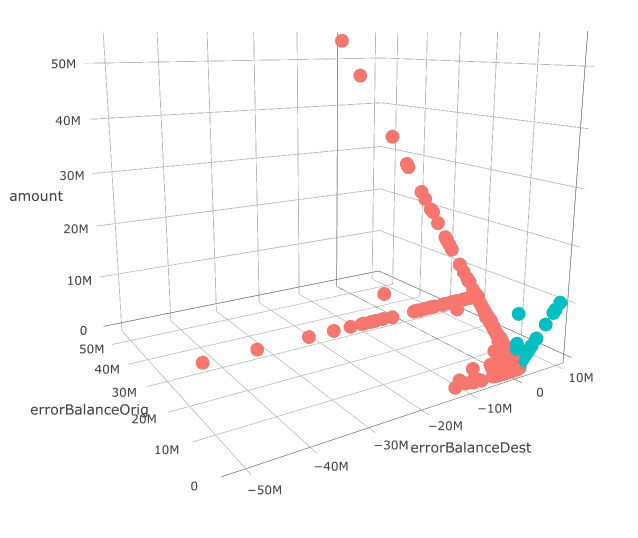
\includegraphics[width=0.7\textwidth,height=\textheight]{figures/paySim/descriptive/threedimensionalplot.png}
\caption{PaySim: Amount, errorBalanceORig and errorBalanceDest plot}
\end{figure}

The framework for fitting the chosen ML techniques is as before, a
10-fold Cross-Validation. It should be noted though, that for this
dataset we have used a variaton of the Logistic Regression, the
Bias-Reduced Logistic Regression, due to the encountered of perfect
separation when working with the original model.

\begin{table}

\caption{\label{tab:paySim_models_AUC}PaySim: AUC Metric Model Variations}
\centering
\resizebox{\textwidth}{!}{\begin{tabular}[t]{lrrrrrrr}
\toprule
type & original & original\_radial & weighted & weighted\_radial & down & up & SMOTE\\
\midrule
Random Forest & 0.9999954 & NA & 0.9999954 & NA & 0.9985756 & 0.9999942 & 0.9994483\\
xGBoost & 0.9999994 & NA & 0.9999994 & NA & 0.9997519 & 0.9999960 & 0.9996079\\
GBM & 0.8795264 & NA & 0.9999931 & NA & 0.9927406 & 0.9999954 & 0.9995275\\
ANN & 0.9968546 & NA & 0.9797525 & NA & 0.9797114 & 0.9713769 & 0.9902082\\
Log. Regression & 0.8717525 & NA & NA & NA & 0.8370850 & 0.9939988 & 0.8717525\\
SVM & 0.9560930 & 0.8788596 & 0.9553215 & 0.8767621 & 0.8765614 & 0.9686560 & 0.9004314\\
\bottomrule
\end{tabular}}
\end{table}

\begin{table}

\caption{\label{tab:paySim_model_PR}PaySim: PR Metric Model Variations}
\centering
\resizebox{\textwidth}{!}{\begin{tabular}[t]{lrrrrrrr}
\toprule
type & original & original\_radial & weighted & weighted\_radial & down & up & SMOTE\\
\midrule
Random Forest & 0.9983619 & NA & 0.9983619 & NA & 0.7850739 & 0.9980407 & 0.8255387\\
xGBoost & 0.9998013 & NA & 0.9998013 & NA & 0.9430914 & 0.9985762 & 0.9109428\\
GBM & 0.5634932 & NA & 0.9974719 & NA & 0.6816623 & 0.9983664 & 0.9108737\\
ANN & 0.9548565 & NA & 0.9452027 & NA & 0.5943965 & 0.5458254 & 0.5087932\\
Log. Regression & 0.0168379 & NA & NA & NA & 0.0205172 & 0.6795277 & 0.0168379\\
SVM & 0.7013130 & 0.0511329 & 0.7026728 & 0.0493418 & 0.5328521 & 0.7623474 & 0.5677162\\
\bottomrule
\end{tabular}}
\end{table}

In tables 8 and 9, we can observe that all models have performed really
well. Nonetheless, we can once more see how the decision tree based
models, Random Forest, xGBoost and GBM are slightly ahead than all the
rest. This is not very evident when looking at the ROC AUC metric, but
it is more pronounced when we shift our view to the Precision-Recall
AUC. It is interesting to see that despite the severe class imbalance,
the SVM models has managed to produced some impressive results. It best
performance is on the dataset with RUS applied on it, meaning that the
imbalance ratio was brought down by generating copies of the minoriy
class observations. Nonetheless, even it its other variations,
especially the cost-sensitive variant with the linear kernel, it has
shown better than expected results.

Both plots on Figure 10 look quite impressive, as most lines are
``hugging'' the upper left or right corner for the ROC and
Precision-Recall cases respectively.

\begin{figure}
\centering
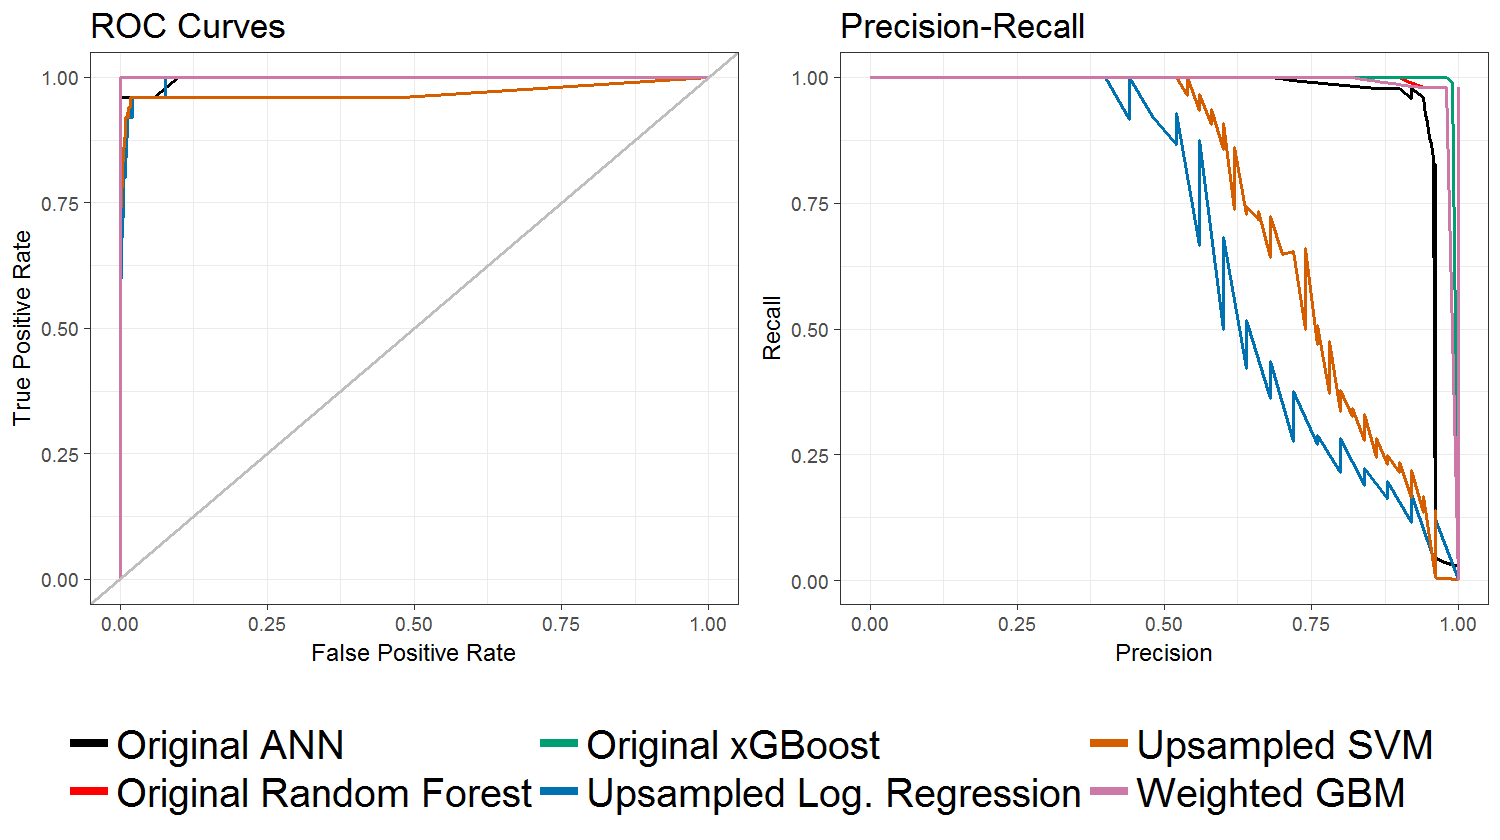
\includegraphics[width=1\textwidth,height=\textheight]{figures/paySim/paySim_pr_roc.png}
\caption{PaySim: ROC and PR Curves}
\end{figure}

\hypertarget{further-improvements}{%
\section{6. Further Improvements}\label{further-improvements}}

We have given a big overview on the different Machine Learning
Techniques that can be used for Financial Fraud Detection. However, in
this paper we have not delved into the details for each individual
algorithm and we have explored only a part of the tunning opportunities
that each algorithm offers. For instance, the ANN models can be extended
to include more than just a single hidden layer or another variation of
it can be tested, i.e.~not the ``vanilla'' model. For GBM and xGBoost, a
wider scope of tuning parameters can be used, which is of course
associated with the need of greater computational power.

\hypertarget{conclusion}{%
\section{7. Conclusion}\label{conclusion}}

\hypertarget{references}{%
\section*{8. References}\label{references}}
\addcontentsline{toc}{section}{8. References}

\hypertarget{refs}{}
\leavevmode\hypertarget{ref-fraudanalyticsacl}{}%
ACL. 2014. ``Fraud Detection Using Data Analytics in the Banking
Industry.'' 2014.
\url{https://www.acl.com/pdfs/DP_Fraud_detection_BANKING.pdf}.

\leavevmode\hypertarget{ref-akbani2004applying}{}%
Akbani, Rehan, Stephen Kwek, and Nathalie Japkowicz. 2004. ``Applying
Support Vector Machines to Imbalanced Datasets.'' In \emph{European
Conference on Machine Learning}, 39--50. Springer.

\leavevmode\hypertarget{ref-batuwita2013class}{}%
Batuwita, Rukshan, and Vasile Palade. 2013. ``Class Imbalance Learning
Methods for Support Vector Machines.''

\leavevmode\hypertarget{ref-buanuarescu2015detecting}{}%
Bănărescu, Adrian. 2015. ``Detecting and Preventing Fraud with Data
Analytics.'' \emph{Procedia Economics and Finance} 32.
Elsevier:1827--36.

\leavevmode\hypertarget{ref-bhardwaj2016financial}{}%
Bhardwaj, Aastha, and Rajan Gupta. 2016. ``Financial Frauds: Data Mining
Based Detection-a Comprehensive Survey.'' \emph{International Journal of
Computer Applications} 156 (10). Foundation of Computer Science.

\leavevmode\hypertarget{ref-bhattacharyya2011data}{}%
Bhattacharyya, Siddhartha, Sanjeev Jha, Kurian Tharakunnel, and J
Christopher Westland. 2011. ``Data Mining for Credit Card Fraud: A
Comparative Study.'' \emph{Decision Support Systems} 50 (3).
Elsevier:602--13.

\leavevmode\hypertarget{ref-bolton2001unsupervised}{}%
Bolton, Richard J, and David J Hand. 2001. ``Unsupervised Profiling
Methods for Fraud Detection.'' \emph{Credit Scoring and Credit Control
VII}. Citeseer, 235--55.

\leavevmode\hypertarget{ref-brause1999neural}{}%
Brause, R, T Langsdorf, and Michael Hepp. 1999. ``Neural Data Mining for
Credit Card Fraud Detection.'' In \emph{Tools with Artificial
Intelligence, 1999. Proceedings. 11th Ieee International Conference on},
103--6. IEEE.

\leavevmode\hypertarget{ref-breiman2001random}{}%
Breiman, Leo. 2001. ``Random Forests.'' \emph{Machine Learning} 45 (1).
Springer:5--32.

\leavevmode\hypertarget{ref-chaudhary2012credit}{}%
Chaudhary, Khyati, and Bhawna Mallick. 2012. ``Credit Card Fraud: The
Study of Its Impact and Detection Techniques.'' Citeseer.

\leavevmode\hypertarget{ref-chawla2002smote}{}%
Chawla, Nitesh V, Kevin W Bowyer, Lawrence O Hall, and W Philip
Kegelmeyer. 2002. ``SMOTE: Synthetic Minority over-Sampling Technique.''
\emph{Journal of Artificial Intelligence Research} 16:321--57.

\leavevmode\hypertarget{ref-chen2016xgboost}{}%
Chen, Tianqi, and Carlos Guestrin. 2016. ``Xgboost: A Scalable Tree
Boosting System.'' In \emph{Proceedings of the 22nd Acm Sigkdd
International Conference on Knowledge Discovery and Data Mining},
785--94. ACM.

\leavevmode\hypertarget{ref-cortes1995support}{}%
Cortes, Corinna, and Vladimir Vapnik. 1995. ``Support-Vector Networks.''
\emph{Machine Learning} 20 (3). Springer:273--97.

\leavevmode\hypertarget{ref-dal2015adaptive}{}%
Dal Pozzolo, Andrea, and Gianluca Bontempi. 2015. ``Adaptive Machine
Learning for Credit Card Fraud Detection.'' Université libre de
Bruxelles.

\leavevmode\hypertarget{ref-dal2015calibrating}{}%
Dal Pozzolo, Andrea, Olivier Caelen, Reid A Johnson, and Gianluca
Bontempi. 2015. ``Calibrating Probability with Undersampling for
Unbalanced Classification.'' In \emph{Computational Intelligence, 2015
Ieee Symposium Series on}, 159--66. IEEE.

\leavevmode\hypertarget{ref-dal2014learned}{}%
Dal Pozzolo, Andrea, Olivier Caelen, Yann-Ael Le Borgne, Serge
Waterschoot, and Gianluca Bontempi. 2014. ``Learned Lessons in Credit
Card Fraud Detection from a Practitioner Perspective.'' \emph{Expert
Systems with Applications} 41 (10). Elsevier:4915--28.

\leavevmode\hypertarget{ref-davis2006relationship}{}%
Davis, Jesse, and Mark Goadrich. 2006. ``The Relationship Between
Precision-Recall and Roc Curves.'' In \emph{Proceedings of the 23rd
International Conference on Machine Learning}, 233--40. ACM.

\leavevmode\hypertarget{ref-dorronsoro1997neural}{}%
Dorronsoro, Jose R, Francisco Ginel, C Sgnchez, and CS Cruz. 1997.
``Neural Fraud Detection in Credit Card Operations.'' \emph{IEEE
Transactions on Neural Networks} 8 (4). IEEE:827--34.

\leavevmode\hypertarget{ref-everett2003credit}{}%
Everett, Catherine. 2003. ``Credit Card Fraud Funds Terrorism.''
\emph{Computer Fraud \& Security} 2003 (5). Elsevier:1.

\leavevmode\hypertarget{ref-analytics_tools_table}{}%
EY. 2014. ``Big Risks Require Big Data Thinking.'' 2014.
\url{http://www.ey.com/Publication/vwLUAssets/EY-Global-Forensic-Data-Analytics-Survey-2014/$FILE/EY-Global-Forensic-Data-Analytics-Survey-2014.pdf}.

\leavevmode\hypertarget{ref-fich2007financial}{}%
Fich, Eliezer M, and Anil Shivdasani. 2007. ``Financial Fraud, Director
Reputation, and Shareholder Wealth.'' \emph{Journal of Financial
Economics} 86 (2). Elsevier:306--36.

\leavevmode\hypertarget{ref-fletcher2007challenges}{}%
Fletcher, Nigel. 2007. ``Challenges for Regulating Financial Fraud in
Cyberspace.'' \emph{Journal of Financial Crime} 14 (2). Emerald Group
Publishing Limited:190--207.

\leavevmode\hypertarget{ref-freund1997decision}{}%
Freund, Yoav, and Robert E Schapire. 1997. ``A Decision-Theoretic
Generalization of on-Line Learning and an Application to Boosting.''
\emph{Journal of Computer and System Sciences} 55 (1). Elsevier:119--39.

\leavevmode\hypertarget{ref-friedman2001greedy}{}%
Friedman, Jerome H. 2001. ``Greedy Function Approximation: A Gradient
Boosting Machine.'' \emph{Annals of Statistics}. JSTOR, 1189--1232.

\leavevmode\hypertarget{ref-friedman2002stochastic}{}%
---------. 2002. ``Stochastic Gradient Boosting.'' \emph{Computational
Statistics \& Data Analysis} 38 (4). Elsevier:367--78.

\leavevmode\hypertarget{ref-friedman2001elements}{}%
Friedman, Jerome, Trevor Hastie, and Robert Tibshirani. 2001. \emph{The
Elements of Statistical Learning}. Vol. 1. Springer series in statistics
New York.

\leavevmode\hypertarget{ref-friedman2000additive}{}%
Friedman, Jerome, Trevor Hastie, Robert Tibshirani, and others. 2000.
``Additive Logistic Regression: A Statistical View of Boosting (with
Discussion and a Rejoinder by the Authors).'' \emph{The Annals of
Statistics} 28 (2). Institute of Mathematical Statistics:337--407.

\leavevmode\hypertarget{ref-ghosh1994credit}{}%
Ghosh, Sushmito, and Douglas L Reilly. 1994. ``Credit Card Fraud
Detection with a Neural-Network.'' In \emph{System Sciences, 1994.
Proceedings of the Twenty-Seventh Hawaii International Conference on},
3:621--30. IEEE.

\leavevmode\hypertarget{ref-grabosky2001electronic}{}%
Grabosky, Peter, Russell G Smith, and Gillian Dempsey. 2001.
\emph{Electronic Theft: Unlawful Acquisition in Cyberspace}. Cambridge
University Press.

\leavevmode\hypertarget{ref-he2009learning}{}%
He, Haibo, and Edwardo A Garcia. 2009. ``Learning from Imbalanced
Data.'' \emph{IEEE Transactions on Knowledge and Data Engineering} 21
(9). Ieee:1263--84.

\leavevmode\hypertarget{ref-james2013introduction}{}%
James, Gareth, Daniela Witten, Trevor Hastie, and Robert Tibshirani.
2013. \emph{An Introduction to Statistical Learning}. Vol. 112.
Springer.

\leavevmode\hypertarget{ref-japkowicz2013assessment}{}%
Japkowicz, Nathalie. 2013. ``Assessment Metrics for Imbalanced
Learning.'' \emph{Imbalanced Learning: Foundations, Algorithms, and
Applications}. Wiley Online Library, 187--206.

\leavevmode\hypertarget{ref-johnson2014learning}{}%
Johnson, Rie, and Tong Zhang. 2014. ``Learning Nonlinear Functions Using
Regularized Greedy Forest.'' \emph{IEEE Transactions on Pattern Analysis
and Machine Intelligence} 36 (5). IEEE:942--54.

\leavevmode\hypertarget{ref-khoshgoftaar2007empirical}{}%
Khoshgoftaar, Taghi M, Moiz Golawala, and Jason Van Hulse. 2007. ``An
Empirical Study of Learning from Imbalanced Data Using Random Forest.''
In \emph{Tools with Artificial Intelligence, 2007. ICTAI 2007. 19th Ieee
International Conference on}. Vol. 2. IEEE.

\leavevmode\hypertarget{ref-laudon2013commerce}{}%
Laudon, Kenneth C, and Carol Guercio Traver. 2013. \emph{E-Commerce}.
Pearson.

\leavevmode\hypertarget{ref-lopez2014social}{}%
Lopez-Rojas, Edgar Alonso, and Stefan Axelsson. 2014. ``Social
Simulation of Commercial and Financial Behaviour for Fraud Detection
Research.'' In \emph{Social Simulation Conference. Bellaterra,
Cerdanyola Del Valles, 1a: 2014}.

\leavevmode\hypertarget{ref-mcalearney2008ignore}{}%
McAlearney, S, and TJX Data Breach. 2008. ``Ignore Cost Lessons and
Weep.'' \emph{CIO, August} 7.

\leavevmode\hypertarget{ref-meyer2003support}{}%
Meyer, David, Friedrich Leisch, and Kurt Hornik. 2003. ``The Support
Vector Machine Under Test.'' \emph{Neurocomputing} 55 (1-2).
Elsevier:169--86.

\leavevmode\hypertarget{ref-natekin2013gradient}{}%
Natekin, Alexey, and Alois Knoll. 2013. ``Gradient Boosting Machines, a
Tutorial.'' \emph{Frontiers in Neurorobotics} 7. Frontiers:21.

\leavevmode\hypertarget{ref-ngai2011application}{}%
Ngai, EWT, Yong Hu, YH Wong, Yijun Chen, and Xin Sun. 2011. ``The
Application of Data Mining Techniques in Financial Fraud Detection: A
Classification Framework and an Academic Review of Literature.''
\emph{Decision Support Systems} 50 (3). Elsevier:559--69.

\leavevmode\hypertarget{ref-nielsen2016tree}{}%
Nielsen, Didrik. 2016. ``Tree Boosting with Xgboost-Why Does Xgboost
Win" Every" Machine Learning Competition?'' Master's thesis, NTNU.

\leavevmode\hypertarget{ref-nilson2016nilson}{}%
Nilson, Spencer. 2016. ``The Nilson Report.''
\url{https://nilsonreport.com/publication_newsletter_archive_issue.php?issue=1096}.

\leavevmode\hypertarget{ref-capitaloneguide}{}%
One, Capital. 2010. ``Identity Theft Guide.'' 2010.
\url{https://www.capitalone.ca/media/doc/canada/identity-theft-guide.pdf}.

\leavevmode\hypertarget{ref-seeja2014fraudminer}{}%
Seeja, KR, and Masoumeh Zareapoor. 2014. ``FraudMiner: A Novel Credit
Card Fraud Detection Model Based on Frequent Itemset Mining.'' \emph{The
Scientific World Journal} 2014. Hindawi.

\leavevmode\hypertarget{ref-van2007experimental}{}%
Van Hulse, Jason, Taghi M Khoshgoftaar, and Amri Napolitano. 2007.
``Experimental Perspectives on Learning from Imbalanced Data.'' In
\emph{Proceedings of the 24th International Conference on Machine
Learning}, 935--42. ACM.

\leavevmode\hypertarget{ref-veropoulos1999controlling}{}%
Veropoulos, Konstantinos, Colin Campbell, Nello Cristianini, and others.
1999. ``Controlling the Sensitivity of Support Vector Machines.'' In
\emph{Proceedings of the International Joint Conference on Ai}, 55:60.

\leavevmode\hypertarget{ref-whiting2012machine}{}%
Whiting, David G, James V Hansen, James B McDonald, Conan Albrecht, and
W Steve Albrecht. 2012. ``Machine Learning Methods for Detecting
Patterns of Management Fraud.'' \emph{Computational Intelligence} 28
(4). Wiley Online Library:505--27.

\leavevmode\hypertarget{ref-whitrow2009transaction}{}%
Whitrow, Christopher, David J Hand, Piotr Juszczak, D Weston, and Niall
M Adams. 2009. ``Transaction Aggregation as a Strategy for Credit Card
Fraud Detection.'' \emph{Data Mining and Knowledge Discovery} 18 (1).
Springer:30--55.


\end{document}
